% \subsubsection{Thiết kế hệ thống}
% Nhằm đảm bảo hệ thống có khả năng bảo trì, mở rộng và kiểm thử dễ dàng, kiến trúc của dự án được thiết kế theo mô hình \textbf{Layered Architecture}. Đây là một mô hình kiến trúc phổ biến và vững chắc, giúp tách bạch rõ ràng các mối quan tâm của ứng dụng thành các lớp logic riêng biệt. Luồng xử lý chính của hệ thống tuân theo quy tắc phụ thuộc chặt chẽ: một lớp ở trên chỉ có thể giao tiếp với lớp ngay bên dưới nó. Dữ liệu yêu cầu sẽ đi từ lớp trên cùng xuống các lớp dưới để xử lý và truy xuất dữ liệu, sau đó dữ liệu phản hồi sẽ được trả ngược lên trên.
% \begin{figure}[H]
%     \centering
%     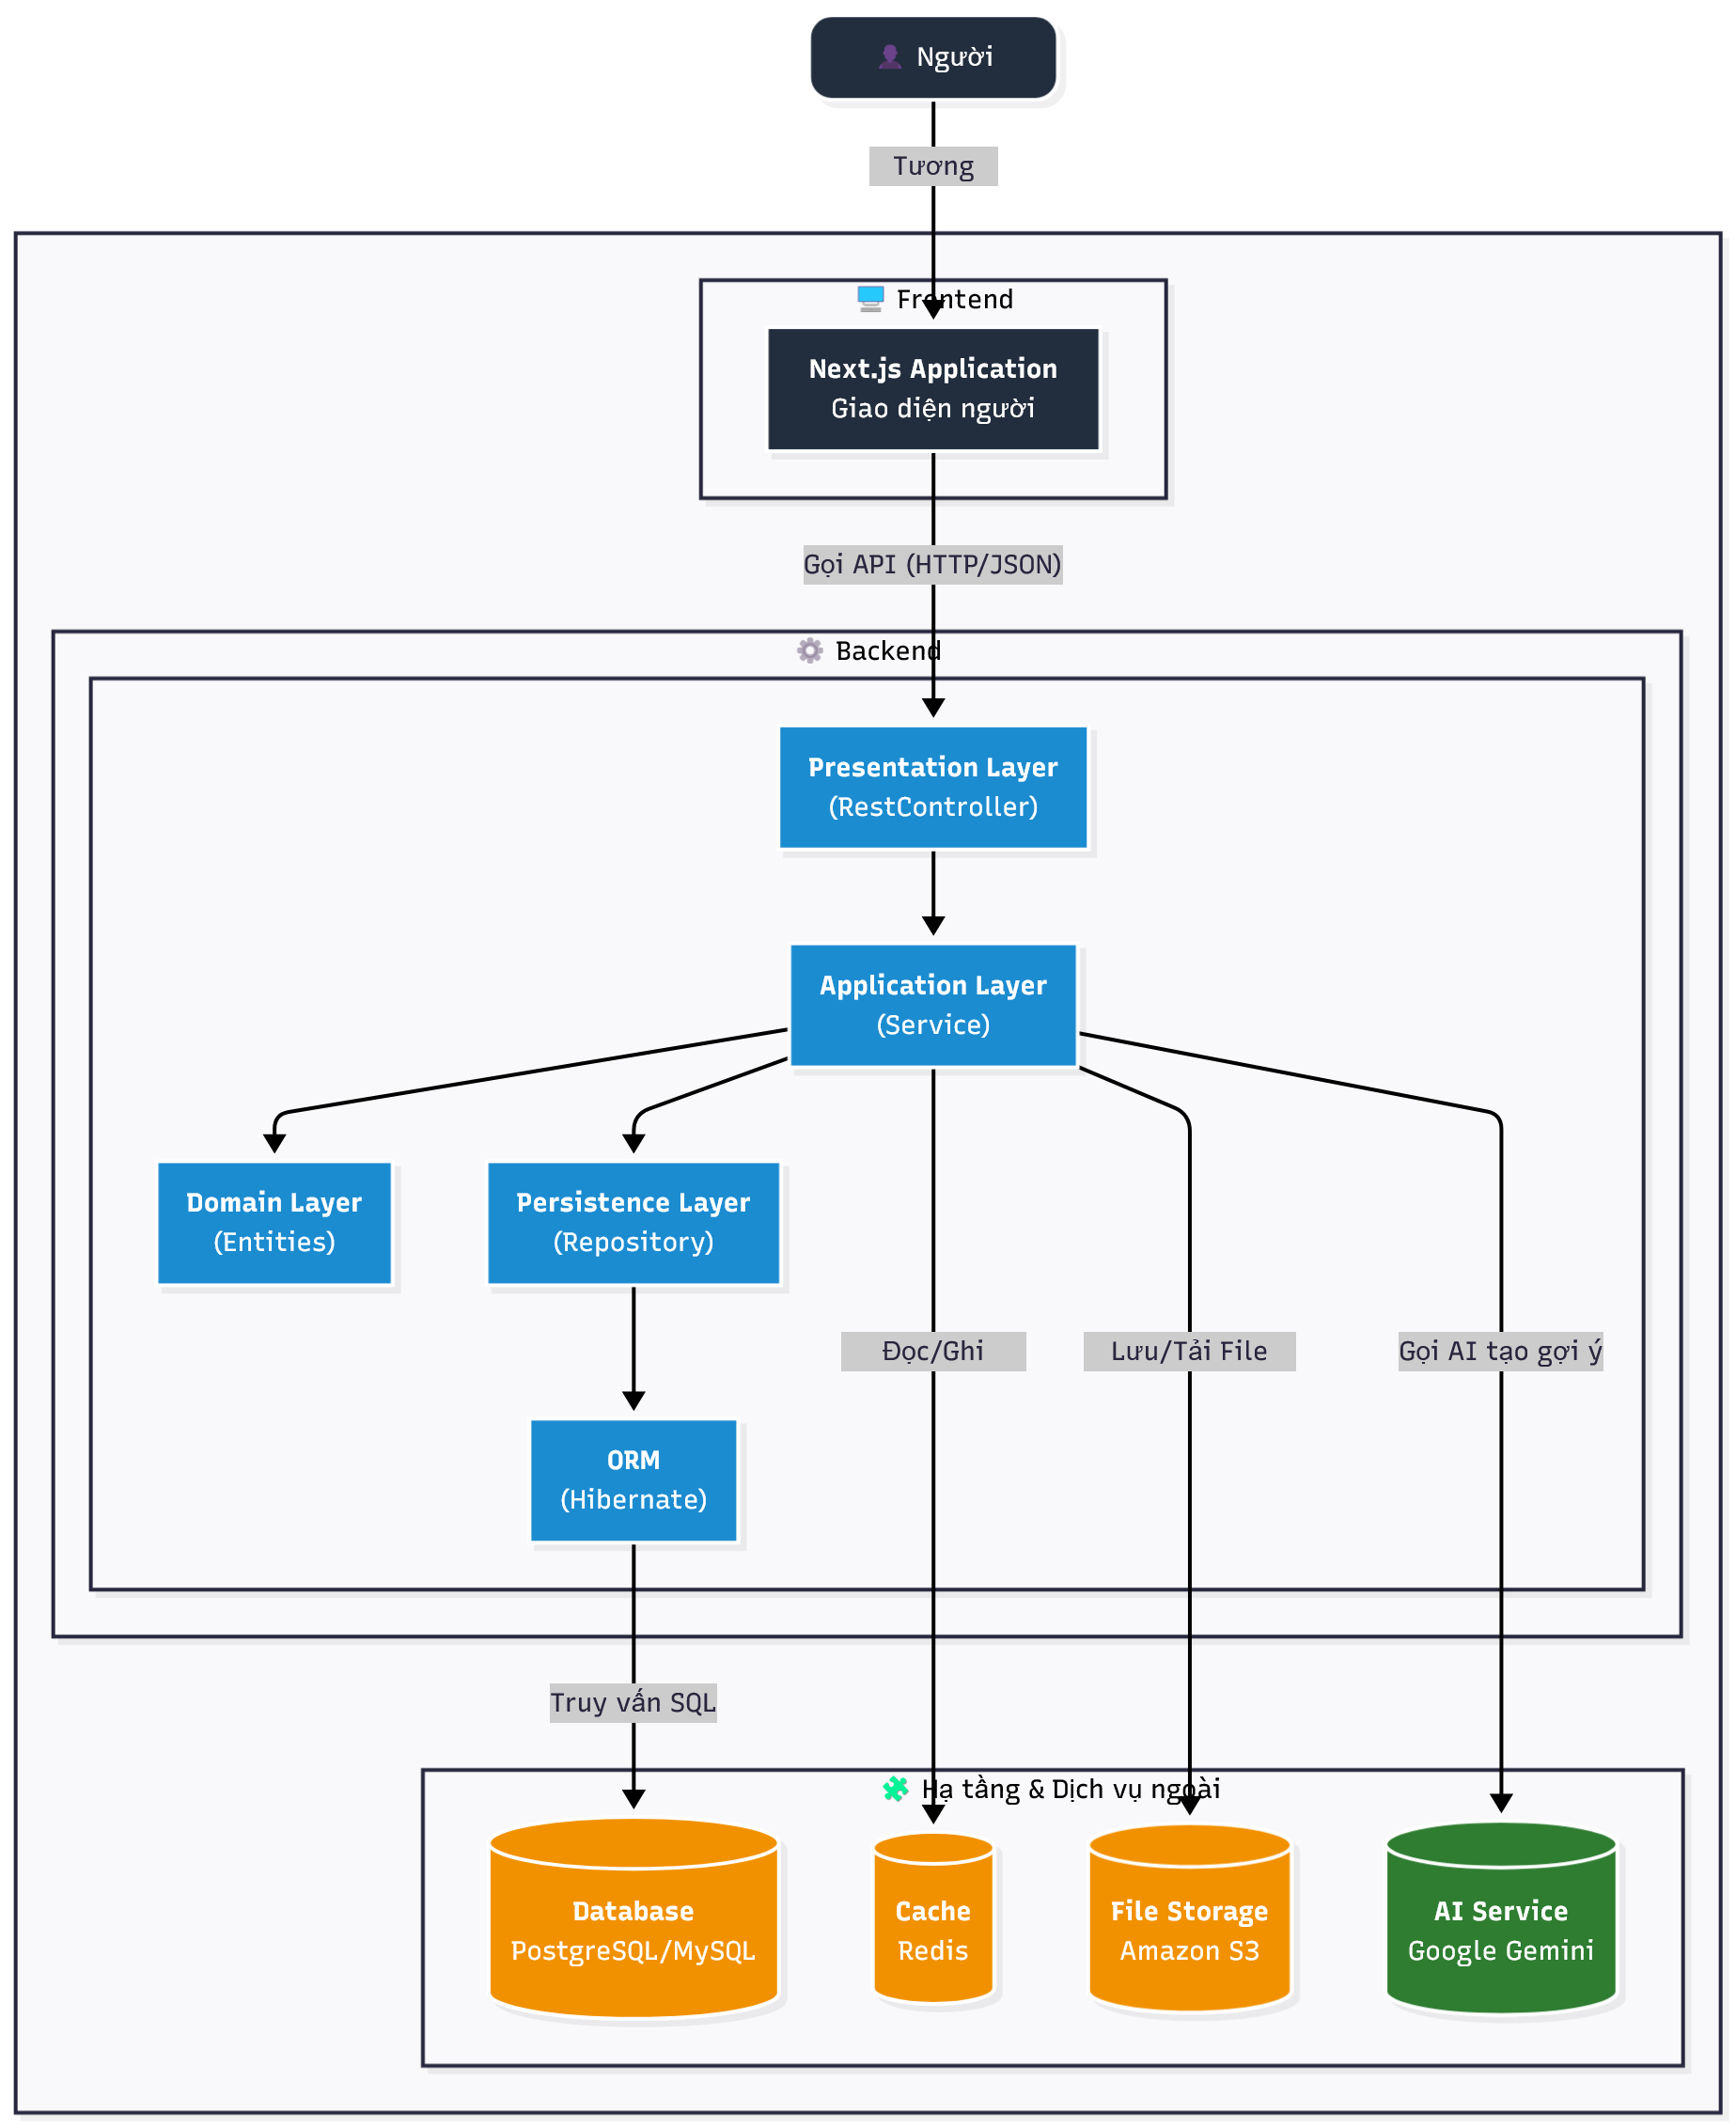
\includegraphics[width=0.9\textwidth]{Images/7. System Design/Kiến trúc hệ thống.png}
%     \caption{Kiến trúc hệ thống}
%     \label{fig:overview_system}
% \end{figure}
% Các tầng trong kiến trúc hệ thống:
% \begin{itemize}
%     \item \textbf{User Interface:} hiển thị giao diện và tiếp nhận tương tác trực tiếp từ người dùng.
%     \item \textbf{Presentation Layer:} tiếp nhận, xác thực và điều hướng các yêu cầu (HTTP/WebSocket) từ client.
%     \item \textbf{Application Layer:} thực thi logic nghiệp vụ chính và điều phối các tác vụ của hệ thống.
%     \item \textbf{Domain Layer:} định nghĩa các thực thể, quy tắc và mô hình kinh doanh cốt lõi.
%     \item \textbf{Persistence Layer :} trừu tượng hóa các hoạt động truy xuất dữ liệu thông qua các interfaces.
%     \item \textbf{Infrastructure Layer:} cung cấp các chức năng kỹ thuật và giao tiếp với các hệ thống bên ngoài (AI, Cache, Email...).
%     \item \textbf{Data Layer:} Lưu trữ vật lý toàn bộ dữ liệu của ứng dụng.
% \end{itemize}

\subsubsection{Mô hình kiến trúc}

\noindent\textbf{a. Giới thiệu:}\par
Hệ thống TravelEZ được thiết kế dựa trên \textbf{Kiến trúc Phân lớp (Layered Architecture)}.
Đây là một mô hình thiết kế phần mềm nền tảng, tổ chức ứng dụng thành các lớp (layers) logic xếp chồng.
Mỗi lớp đảm nhiệm một vai trò và trách nhiệm chuyên biệt. Mô hình này áp dụng một quy tắc phụ thuộc chặt chẽ:
một lớp ở trên chỉ được phép giao tiếp với lớp ngay bên dưới nó.

Trong hệ thống TravelEZ, kiến trúc này được áp dụng để phân định rạch ròi các khối chức năng chính:
\begin{enumerate}
    \item \textbf{Giao diện người dùng (Frontend):} Xây dựng bằng Next.js, chịu trách nhiệm hoàn toàn về việc hiển thị dữ liệu và tiếp nhận tương tác từ người dùng cuối.
    \item \textbf{Logic Nghiệp vụ (Backend):} Xây dựng bằng Spring Boot, là lõi xử lý toàn bộ các nghiệp vụ phức tạp của hệ thống.
    \item \textbf{Hạ tầng và Dữ liệu (Infrastructure \& Data):} Bao gồm các dịch vụ kỹ thuật và lưu trữ bên ngoài như Database (PostgreSQL), Cache (Redis), Lưu trữ file (Amazon S3) và Dịch vụ AI (Google Gemini).
\end{enumerate}

\noindent\textbf{b. Ưu điểm:}\par
Việc lựa chọn Kiến trúc Phân lớp (với Frontend/Backend tách biệt) mang lại các lợi ích kỹ thuật trực tiếp cho việc phát triển hệ thống TravelEZ:
\begin{itemize}
    \item \textbf{Tính Mô-đun và Phân tách Trách nhiệm (Modularity \& Separation of Concerns):}
    Đây là ưu điểm cốt lõi. Logic nghiệp vụ (ở Application Layer) không bị phụ thuộc vào cách nó được hiển thị (Frontend)
    hay cách nó được lưu trữ (Persistence Layer). Điều này cho phép thay thế hoặc nâng cấp một thành phần mà không phá vỡ
    các thành phần khác.

    \item \textbf{Tăng cường khả năng bảo trì:}
    Khi có lỗi phát sinh, kiến trúc này cho phép khoanh vùng vấn đề dễ dàng hơn
    (ví dụ: lỗi hiển thị ở Frontend, lỗi logic ở Application, hoặc lỗi truy vấn ở Persistence).
    Mã nguồn trở nên rõ ràng và dễ quản lý hơn khi hệ thống phát triển về quy mô.

    \item \textbf{Khả năng kiểm thử (Testability):}
    Cấu trúc phân lớp cho phép thực hiện kiểm thử đơn vị (unit test) một cách độc lập cho từng lớp.
    Ví dụ, có thể kiểm thử Application Layer bằng cách "mock" (giả lập) Persistence Layer,
    đảm bảo logic nghiệp vụ hoạt động chính xác mà không cần phụ thuộc vào cơ sở dữ liệu thật.

    \item \textbf{Khả năng tái sử dụng (Reusability):}
    Lớp Application Layer và Domain Layer, vốn chứa đựng nghiệp vụ lõi, có thể được tái sử dụng hoàn toàn.
    Nếu hệ thống cần hỗ trợ thêm một kênh giao tiếp mới (ví dụ: ứng dụng di động),
    chỉ cần xây dựng một giao diện mới (tương tự Frontend) mà không cần viết lại logic nghiệp vụ.
\end{itemize}

\noindent\textbf{c. So sánh với các mô hình kiến trúc khác}\par
% Bảng \ref{tab:so_sanh_kien_truc} phân tích các lựa chọn kiến trúc dựa trên các tiêu chí kỹ thuật thuần túy:

\begin{table}[h!]
    \centering
    
    \resizebox{\textwidth}{!}{%
    \begin{tabular}{|l|p{4cm}|p{4cm}|p{4cm}|p{4cm}|}
        \hline
        \textbf{Tiêu chí} & \textbf{Kiến trúc Phân lớp (Layered)} & \textbf{Kiên trúc Vi dịch vụ (Microservices)} & \textbf{Kiến trúc Hướng sự kiện (Event-Driven)} & \textbf{Kiến trúc Đơn khối (Monolithic - không phân lớp)} \\
        \hline
        \textbf{Độ phức tạp} & \textbf{Trung bình:} Yêu cầu quản lý hai codebase (Frontend, Backend) và giao tiếp API. Tuy nhiên, cấu trúc mỗi phần rõ ràng. & \textbf{Rất cao:} Đòi hỏi quản lý giao tiếp liên dịch vụ, cơ sở hạ tầng phức tạp (service discovery, API gateway). & \textbf{Cao:} Đòi hỏi tư duy bất đồng bộ, cần hệ thống message broker (như RabbitMQ, Kafka). Khó theo dõi luồng logic. & \textbf{Thấp (ban đầu):} Dễ bắt đầu, nhưng độ phức tạp tăng nhanh, dẫn đến hệ thống khó kiểm soát (big ball of mud). \\
        \hline
        \textbf{Khả năng bảo trì} & \textbf{Tốt:} Các lớp được tách biệt rõ ràng. Dễ dàng tìm và sửa lỗi trong một lớp cụ thể (ví dụ: lỗi logic ở Application Layer). & \textbf{Rất cao (ở cấp độ dịch vụ):} Có thể sửa, nâng cấp, triển khai lại một dịch vụ (ví dụ: dịch vụ review) mà không ảnh hưởng đến phần còn lại. & \textbf{Trung bình:} Rất linh hoạt, các module hoàn toàn độc lập (decoupled). Nhưng rất khó gỡ lỗi (debug) một chuỗi sự kiện. & \textbf{Rất thấp:} Các thành phần liên kết chặt chẽ (tight coupling). Sửa một chỗ có thể làm hỏng nhiều chỗ khác. \\
        \hline
        \textbf{Khả năng mở rộng} & \textbf{Tốt:} Có thể mở rộng (scale) Frontend và Backend một cách độc lập tùy theo tải. & \textbf{Rất cao:} Có thể mở rộng (scale) từng dịch vụ một cách độc lập (ví dụ: tăng gấp 10 lần dịch vụ 'Gợi ý AI' khi có nhiều người dùng). & \textbf{Rất cao:} Các dịch vụ xử lý sự kiện có thể được mở rộng độc lập, lý tưởng cho các tác vụ tốn thời gian (như gửi thông báo). & \textbf{Thấp:} Phải mở rộng toàn bộ ứng dụng. \\
        \hline
        \textbf{Khả năng kiểm thử} & \textbf{Tốt:} Có thể kiểm thử Backend (API) và Frontend độc lập. Kiểm thử logic ở Application Layer dễ dàng bằng cách mock Persistence Layer. & \textbf{Phức tạp:} Cần kiểm thử tích hợp (integration testing) giữa các dịch vụ, tốn nhiều công sức. & \textbf{Phức tạp:} Kiểm thử đơn vị (unit test) thì dễ, nhưng kiểm thử luồng tích hợp (toàn bộ chuỗi sự kiện) là một thách thức lớn. & \textbf{Rất khó:} Khó cô lập các thành phần để kiểm thử. \\
        \hline
    \end{tabular}%
    }

    \caption{Phân tích so sánh các mô hình kiến trúc}
    \label{tab:so_sanh_kien_truc}
\end{table}
